\section{Introduction}

\subsection{Background}
Over the past few years, a number of communities on the West Coast of
Scotland have build wireless networks whose capacity greatly exceeds the 
bandwidth available in neighbouring areas from commercial suppliers.
Although, there are plans to provide new points of presence under the
Scottish Government's Step Change programme, the estimates of when
these will be on line vary, and there are no details of what will be
available and at what cost.  Moreover many communities will remain out
of reach of the indicated points of presence. Roughly speaking, anyone
whose internet connection travels over more than a mile or so of
copper will see little improvement from the Step Change programme.

The proposal is to construct a high-speed ``backbone'' to serve these
community networks. It will connect to existing fibre and will have
links to the new points of presence as they become available.

This network can be built now without waiting for the completion of the Step Change programme and as the main roll-out proceeds it will only become more useful and enable new connections to the new fibre network,  if and when affordable access is available.  It will provide greater resilience against failure and reach further communities that will not benefit from the current roll-out.

The proposed backbone and coverage is shown in the following figure.
It covers an area stretching over 125km from Loch Torridon to Mull.
Currently the only places in this area at which one can purchase
bandwidth sufficient to the needs of these communities are Oban and
Fort William.
The first phase would carry a  connection at Fort William (where
connection to fibre is possible) North to Applecross. HebNet has
already pushed through a trial link from Eigg to Fort William.  A
second phase would connect via NW Mull to Eigg for added resilience.  

\begin{itemize}

\item Loch Hourn Broadband Cooperative (the Tegola project), started in 2008 serving Loch Hourn and NW Knoydart
\item Hebnet, started in 2011 serving the Small Isles and S Knoydart
\item Locheilnet, started in 2013 serving areas to the North of Fort William with CBS funding
\item Applenet, serving Applecross, Loch Torridon and
  N. Raasay. Started in 2013, and subsequently received CBS funding
\item Sleat. Under development
\item Achmore.  Under development with CBS funding
\item Glenelg. Under development
\item Strathaird (Elgol, Torrin etc).  Under development
\end{itemize}

 
With sufficient capacity the backbone could also serve
N. Ardnamurchan,  and other areas on the Inner Sound, Loch Duich, and Loch Carron
The initial backbone is shown in Figure~\ref{longlinks} and comprises five long links (in
red).  The second phase(in yellow) , as well as serving North Mull, would have the
potential to serve S. Arnamurchan and parts of Morvern.  This figure
only shows the new links. It does not show the substantial
infrastructure already in place to serve individual communities.  Of
the proposed relay sites in the first phase, only B (Ranachan) is
entirely new.

\begin{figure}
\begin{center}
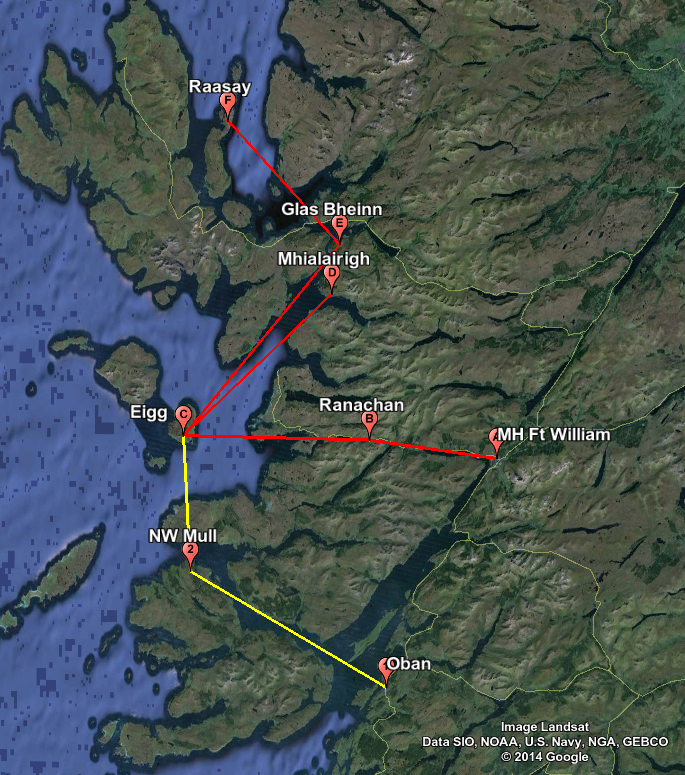
\includegraphics[width=3in]{longlinks.png}
\end{center}
\caption{Overall scheme of the proposed backbone}
\label{longlinks}
\end{figure}




\subsection{Summary of Plan}

There are two major components to this project: (a) building and
maintaining the wireless network infrastructure to connect the
communities with the ``points of presence''  and (b) providing an
internet connection and other services one associates with an ISP at
those points of presence.  Most of the capital costs are associated
with (a); the running costs are roughly similar for (a) and (b)

\subsubsection{The network infrastructure}
The proposed network has to support a bandwidth  that is beyond the
capacity of the relatively inexpensive equipment that is currently
being deployed by community networks.  Moreover the restrictions on
radiated power make it possible to provide that bandwidth only in the
licenced spectra.  The wireless equipment that operates at these
frequencies is  more expensive, bulkier, and requires more power.  At
the same time is is probably more reliable.

The first phase of the plan calls for five of these point-to-point
links. Each point-to point link consists of a pair of radios and and
requires an annual licence fee.  The wireless dishes are larger than
the 60cm diameter ones that are in widespread use by communities. They
will have greater wind resistance and require more accurate
alignment.  This will call for strengthening of the existing relays.
This is a list of the existing and proposed relay sites and a summary
of what needs to be done for phase 1.

It is important to note that using existing commercial towers is
financially prohibitive both for both capital operating expenses

\begin{itemize}
\item[A.] Marine Harvest, Fort William.  This is wher Locheilnet
  already has an internet connection.  Marine Harvest have benefitted
  from, and are supporting community broadband projects.  We believe
  they will be happy to host the link for this larger community
  network.

\item[B.] Ranachan.  This is a surprising location that can ``see''
  both Fort William and Eigg.  It is within 500m of a power line, and
  the only technical difficulty in setting up a relay may be
  access, as it is on the side of a rather steep hillside. We are
  currently seeking permission for Ranachan.  It may be that there are
  local communities that will benefit from a connection.

\item[C.] Eigg.  This is a key relay that already exists.  The current
  power line is over 1km and may need to be upgraded, and the nautical
  arrangement of wire stays will need to be strengthened.

  In addition to serving the Small Isles and Knoydart, Eigg can serve
  N. Ardnamuchan, Glen Uig and some areas on the SW of Skye

\item[D.] Beinn Mhialairigh.  This is a recently constructed relay
  with an adequate power supply.  It will need some additional
  bracing.  The proposed Eigg-Mhialairigh link will replace an
  existing link.

  Mhialarigh will serve Loch Hourn and various areas on the North and
  West of the Sleat peninsula, as well
  as providing a link to the existing network centered on Sabhal M\`or Ostaig.

\item[E.] Glas Bheinn.  A trial relay was erected there in the Spring
  of 2013.  It is in a key position for serving areas to the
  North of Lochalsh.  A rigid structure will have to be created.
  There is good access using an ATV.  The main problem is power.
  While this is being negotiated, we have the possiblity of the loan
  of a substantial solar and wind turbine module.

  Glas Bheinn can serve Loch Carron and areas south of Applecross as
  well as numerous areas around Loch Duich

\item[F.] Raasay.  A relay was erected in 2013 by Applenet.  This may
  need strengthening.  It will serve Applecross and areas to the North
  such as Loch Torridon

\end{itemize}

